\documentclass{article}
\usepackage[T1]{fontenc}
\usepackage{lmodern}
\usepackage{graphicx}
\usepackage{amsmath,amssymb}
\usepackage[a4paper,margin=2cm]{geometry}
\usepackage[absolute,overlay]{textpos}
\setlength{\TPHorizModule}{1mm}
\setlength{\TPVertModule}{1mm}
\usepackage[indonesian]{babel}
\usepackage{hyperref}
\setlength{\emergencystretch}{2em}
% unit: Halaman 1

\begin{document}

% === Halaman 1 (llm) ===

\vspace{84.05mm}

\textbf{IF4020 Kriptografi}

\Huge \textcolor{red}{01 - Pengantar Kriptografi}

\large Oleh: Rinaldi Munir

\vspace{50mm}

\begin{center}
\textbf{Program Studi Teknik Informatika}\
\textbf{Sekolah Teknik Elektro dan Informatika ITB}\
\textbf{2026}
\end{center}

% deskripsi: Ilustrasi konsep kriptografi dengan ikon gembok biru dan kode biner
% bbox normalisasi: [0.7220, 0.0000, 1.0000, 0.2830]
\begin{textblock*}{58.38mm}(151.62mm,0.00mm)
\noindent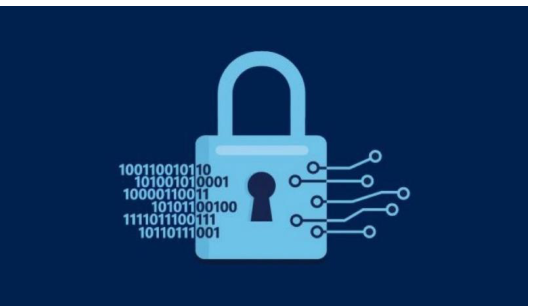
\includegraphics[width=58.38mm,height=84.05mm]{../../images/llm/page_001_img_01.png}%
\end{textblock*}

% deskripsi: Ilustrasi visual enkripsi data berupa label 'data encryption' di atas keyboard komputer
% bbox normalisasi: [0.0000, 0.6500, 0.2670, 0.9990]
\begin{textblock*}{56.07mm}(0.00mm,193.05mm)
\noindent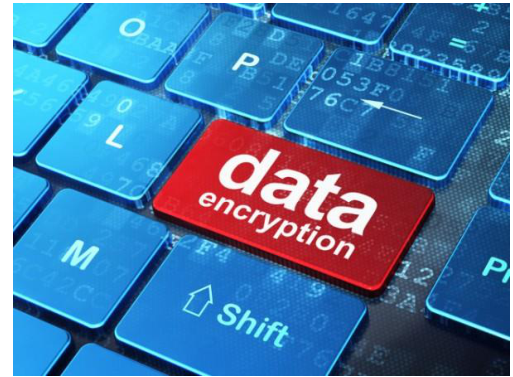
\includegraphics[width=56.07mm,height=103.65mm]{../../images/llm/page_001_img_02.png}%
\end{textblock*}

\end{document}
